\documentclass[11pt,a4paper]{ctexart}
\usepackage[a4paper,margin=1.8cm,headheight=14pt]{geometry}
\usepackage{amsmath,amssymb,mathtools}
\usepackage{booktabs,tabularx,longtable,array,multirow}
\usepackage{enumitem}
\usepackage{tikz}
\usetikzlibrary{arrows.meta,positioning,shapes.geometric,fit,calc}
\usepackage[most]{tcolorbox}
\usepackage{xcolor}
\usepackage{fancyhdr}
\usepackage{hyperref}
\usepackage{microtype}
\setlength{\parindent}{2em}
\setlength{\parskip}{0.35em}
\setlist[itemize]{itemsep=0.2em,topsep=0.3em}
\setlist[enumerate]{itemsep=0.2em,topsep=0.3em}
\hypersetup{colorlinks=true,linkcolor=blue!45!black,urlcolor=blue!50!black}

\definecolor{mainblue}{RGB}{45,86,140}
\definecolor{deepblue}{RGB}{30,62,102}
\definecolor{softblue}{RGB}{238,245,252}
\definecolor{softgreen}{RGB}{238,249,243}
\definecolor{softorange}{RGB}{253,246,233}
\definecolor{softred}{RGB}{253,239,239}
\definecolor{softgray}{RGB}{246,247,249}
\definecolor{deepgreen}{RGB}{35,105,75}
\definecolor{deeporange}{RGB}{165,98,22}
\definecolor{deepred}{RGB}{150,55,55}

\pagestyle{fancy}
\fancyhf{}
\lhead{408 操作系统方法论}
\rhead{进程·线程·调度·系统调用/中断}
\cfoot{\thepage}
\renewcommand{\headrulewidth}{0.4pt}

\newtcolorbox{corebox}[1][]{colback=softblue,colframe=mainblue,title=#1,fonttitle=\bfseries,boxrule=0.8pt,arc=2mm}
\newtcolorbox{exam}[1][]{colback=softorange,colframe=deeporange,title=#1,fonttitle=\bfseries,boxrule=0.8pt,arc=2mm}
\newtcolorbox{warn}[1][]{colback=softred,colframe=deepred,title=#1,fonttitle=\bfseries,boxrule=0.8pt,arc=2mm}
\newtcolorbox{eng}[1][]{colback=softgreen,colframe=deepgreen,title=#1,fonttitle=\bfseries,boxrule=0.8pt,arc=2mm}
\newtcolorbox{method}[1][]{colback=softgray,colframe=black!45,title=#1,fonttitle=\bfseries,boxrule=0.6pt,arc=2mm}

\newcommand{\kw}[1]{\textbf{#1}}
\newcommand{\code}[1]{\texttt{#1}}

\title{\vspace{-1.2cm}\textbf{操作系统问题解决方法论：控制权、进程、线程与调度}\\[0.4em]
\large 以“一个进程的一生”为主线重构 408 核心机制}
\author{408 统一方法论手册 · OS 第一模块}
\date{}

\begin{document}
\maketitle
\begin{corebox}[本章总纲]
这一模块不以“背定义”为主线，而以一个更底层的问题为主线：

\begin{center}
\Large\bfseries 用户程序怎样高速直接运行，而操作系统又始终能够重新取得控制权，\par
并把有限 CPU 时间安全地分给多个执行流？
\end{center}

整章统一为一个受约束状态机：
\[
\boxed{\text{当前状态}+\text{事件}\xrightarrow[\text{策略}]{\text{机制}}\text{新状态}}
\]
且每一步都必须满足保护、隔离、资源所有权与进展性等不变量。
\end{corebox}

\tableofcontents
\newpage

\section{先建立总模型：OS 管的不是“程序”，而是控制权与资源状态}

\subsection{操作系统这一模块的五个母问题}

面对进程、线程、调度、系统调用和中断，不要先背术语。先回答：

\begin{enumerate}
  \item \kw{谁现在拥有 CPU 控制权？} 用户程序还是内核？
  \item \kw{CPU 上真正正在执行的实体是谁？} 一个进程中的哪条执行流？
  \item \kw{这个执行流依附于哪个资源环境？} 地址空间、文件表、权限、信号等属于谁？
  \item \kw{什么事件会迫使执行路径改变？} 系统调用、异常、中断、阻塞、唤醒、抢占、退出。
  \item \kw{当多个执行实体都想运行时，谁来选择下一位？} 调度机制如何获得机会，调度策略如何作选择？
\end{enumerate}

\begin{method}[OS 第一模块统一解题八问]
拿到任何进程/线程/调度题，依次问：
\begin{enumerate}
\item 当前运行实体是谁？
\item 当前处于用户态还是内核态？
\item 发生了什么事件？
\item 这个事件只是\kw{模式切换}，还是会导致\kw{调度/上下文切换}？
\item 当前实体为什么还能继续/为什么必须等待？
\item 若不能继续，它应进入 Ready 还是 Blocked？
\item 哪些资源继续属于它，哪些状态需要保存？
\item 最终谁获得 CPU，代价是什么？
\end{enumerate}
\end{method}

\subsection{两个不能混淆的“状态”}

本模块同时出现两类状态：

\begin{itemize}
  \item \kw{体系结构执行状态}：PC、通用寄存器、SP、状态寄存器等，决定“这条执行流下一步从哪里继续”。
  \item \kw{内核管理状态}：任务状态、调度信息、地址空间引用、打开文件、权限、等待对象等，决定“OS 怎样管理它”。
\end{itemize}

进程/线程切换，本质上就是：\kw{保存旧执行上下文，选择新的可运行实体，再恢复新执行上下文}。

\section{第零章：为什么内核必须先解决“控制权”问题}

\subsection{受限直接执行：又要快，又不能失控}

最简单的高性能方案当然是让用户程序直接在 CPU 上运行：
\[
\text{Program}\rightarrow\text{CPU}
\]
但若程序执行：
\begin{verbatim}
while (1) { }
\end{verbatim}
且 OS 没有任何硬件帮助，它可能永远拿不回 CPU。

因此产生核心矛盾：
\[
\boxed{\text{Direct Execution for Performance}}
\qquad\text{vs.}\qquad
\boxed{\text{Restricted Control for Safety}}
\]
解决它依赖\kw{特权级 + 陷入/返回机制 + 时钟中断}。

\subsection{用户态与内核态：不是“两个程序”，而是权限边界}

CPU 至少区分两类执行权限：

\begingroup
\small
\renewcommand{\arraystretch}{1.25}
\setlength{\tabcolsep}{6pt}
\begin{tabularx}{\linewidth}{>{\bfseries}p{0.26\linewidth} X X}
\toprule
对比维度 & 用户态 (User Mode) & 内核态 (Kernel Mode)\\
\midrule
能否执行特权指令 & 受限（仅非特权指令） & 可以（完整指令集）\\
能否直接配置页表/设备 & 通常不允许（引发硬件异常） & 内核可以（拥有写 CR3 与 I/O 权限）\\
运行的代码 & 普通应用 / 用户函数库 & 内核代码 / 驱动程序\\
设计目标 & 隔离进程、限制非法破坏 & 虚拟化资源、管理全局安全\\
\bottomrule
\end{tabularx}
\endgroup

\begin{corebox}[关键理解]
\kw{用户态/内核态是 CPU 执行权限状态，不等于“当前是不是 OS 进程”。} 同一个用户进程发起系统调用后，可以在\kw{同一进程上下文}中执行内核代码。
\end{corebox}

\subsection{进入内核的三种典型入口}

\begingroup
\small
\renewcommand{\arraystretch}{1.25}
\setlength{\tabcolsep}{5pt}
\begin{tabularx}{\linewidth}{>{\bfseries}p{0.18\linewidth} p{0.12\linewidth} p{0.32\linewidth} X}
\toprule
入口 & 同步性 & 典型来源 & 直观含义与响应动作\\
\midrule
系统调用 & 同步 & 当前程序显式请求 (\code{trap / syscall}) & “我需要内核提供服务”\\
异常/陷阱 & 同步 & 当前指令执行产生 (除零 / 缺页) & “这条指令遇到了特殊硬件情况”\\
外部中断 & 异步 & 定时器、磁盘 I/O、网卡到达 & “外部硬件设备发生了事件”\\
\bottomrule
\end{tabularx}
\endgroup

它们都可能使 CPU 从 user mode 进入 kernel mode，但\kw{原因不同、后续处理也不同}。

\subsection{Trap 之后不一定 Context Switch}

这是本模块第一大易错点。

\begin{center}
\begingroup
\small
\begin{tikzpicture}[>=Stealth, node distance=1.6cm]
\tikzset{
  n/.style={draw=mainblue, thick, fill=softblue, rounded corners=2mm, align=center, minimum width=2.6cm, minimum height=0.85cm, font=\bfseries}
}
\node[n] (u) {进程 A\\用户态};
\node[n, right=of u] (k) {进程 A\\内核态};
\node[n, right=of k] (u2) {进程 A\\用户态};
\draw[->, thick, deepblue] (u) -- node[above=2pt, font=\small] {syscall / trap} (k);
\draw[->, thick, deepblue] (k) -- node[above=2pt, font=\small] {sysret / iret} (u2);
\end{tikzpicture}
\endgroup
\end{center}

这只是：
\[
\boxed{\text{Mode Switch (模式切换)}}
\]

若 A 在内核中因为等待 I/O 不能继续，才可能出现：

\begin{center}
\begingroup
\small
\begin{tikzpicture}[>=Stealth, node distance=1.1cm]
\tikzset{
  n/.style={draw=mainblue, thick, fill=softblue, rounded corners=2mm, align=center, minimum width=2.1cm, minimum height=0.85cm, font=\bfseries}
}
\node[n] (a1) {A 用户态};
\node[n, right=of a1] (a2) {A 内核态};
\node[n, right=of a2, fill=softorange, draw=deeporange] (s) {调度器};
\node[n, right=of s] (b2) {B 内核上下文};
\node[n, right=of b2] (b1) {B 用户态};
\draw[->, thick, deepblue] (a1) -- (a2);
\draw[->, thick, deepblue] (a2) -- node[above=2pt, font=\small] {A 阻塞} (s);
\draw[->, thick, deepblue] (s) -- node[above=2pt, font=\small] {Context Switch} (b2);
\draw[->, thick, deepblue] (b2) -- (b1);
\end{tikzpicture}
\endgroup
\end{center}

这才包含：
\[
\boxed{\text{Context Switch}}
\]

\begin{exam}[408 必须区分]
\begin{itemize}
\item 进入内核态 \(\neq\) 一定切换进程；
\item 发生中断 \(\neq\) 一定进行调度；
\item 进行调度 \(\neq\) 一定切换到不同实体（可能仍选中当前实体）；
\item 阻塞通常意味着当前执行实体暂时不能继续，因此会触发调度机会。
\end{itemize}
\end{exam}

\section{程序、进程与线程：把“资源世界”和“执行路径”拆开}

\subsection{程序是静态蓝图，进程是动态执行环境}

考试层面可以记：\kw{程序是静态的指令和数据集合；进程是程序的一次执行实例。}

但更有用的结构是：
\[
\boxed{\text{Process}=\text{Resource/Protection Context}+\text{one or more Execution Contexts}}
\]

一个典型进程包含：
\begin{itemize}
\item 虚拟地址空间及其页表/映射；
\item 打开的文件描述符与其他内核资源引用；
\item 身份、权限、信号等控制信息；
\item 一个或多个线程所对应的执行上下文。
\end{itemize}

\subsection{线程是执行上下文，而不是第二套资源世界}

线程最稳定的理解是：
\[
\boxed{\text{Thread}=PC+Registers+Stack+Scheduling State+Thread Metadata}
\]

同一进程内线程通常共享：
\[
\text{Code, Global Data, Heap, Address Space, Open Files}
\]
而每个线程至少需要独立维护：
\[
\text{PC, Registers, Stack, Execution/Scheduling State}
\]

\begin{warn}[不要把“线程是调度基本单位”绝对化]
在 408 的现代内核线程模型中，可以把线程理解为 CPU 调度的基本执行实体；但纯用户级线程若内核不可见，内核实际调度的是其承载的内核调度实体。手册中应把“408 教材表达”和“实现边界”分开写。
\end{warn}

\subsection{并发与并行}

\begin{itemize}
\item \kw{Concurrency（并发）}：多个逻辑执行流在一段时间内都取得进展，不要求同一物理时刻同时执行。
\item \kw{Parallelism（并行）}：多个执行流在不同核心/执行单元上物理同时执行。
\end{itemize}

不要把并发仅理解成“单核伪同时”。多核系统同样存在并发，只是部分并发执行流可能同时并行。

\subsection{408 视角下的进程/线程对比}

\begingroup
\small
\renewcommand{\arraystretch}{1.25}
\setlength{\tabcolsep}{6pt}
\begin{tabularx}{\linewidth}{>{\bfseries}p{0.18\linewidth} X X}
\toprule
对比维度 & 进程 (Process) & 同一进程内的线程 (Thread)\\
\midrule
核心角色 & 资源分配与保护环境 & 独立执行路径与 CPU 调度实体\\
地址空间 & 通常彼此独立隔离 & 共享所属进程的整个虚拟地址空间\\
切换开销 & 必须切换页表 (CR3)，开销大 & 同进程线程切换无须切页表，开销小\\
通信机制 & 需要 IPC / 共享内存映射 & 可直接读写共享堆/全局变量（需同步）\\
故障隔离 & 隔离性强，崩溃通常不影响其他进程 & 共享地址空间，致命错误常导致整个进程崩溃\\
\bottomrule
\end{tabularx}
\endgroup

\section{进程拥有的资源到底怎样被内核表示：把 VFS 接入生命周期}

\subsection{不要背“三级表”，先看解耦目标}

进程对文件的使用需要同时满足两个矛盾需求：
\begin{enumerate}
\item 对用户提供非常简单的整数句柄；
\item 允许多个描述符/多个进程共享或独立维护“打开实例”的状态；
\item 最终仍要指向同一个文件系统对象。
\end{enumerate}

因此可以抽象为：
\[
\boxed{\text{fd}\rightarrow\text{Open File Description}\rightarrow\text{Filesystem Object}}
\]
在 Linux VFS 中，常见实现路径进一步表现为：
\[
\boxed{\text{fd table}\rightarrow\texttt{struct file}\rightarrow\text{dentry/inode}\rightarrow\text{data}}
\]

\subsection{第一层：文件描述符表是进程级引用表}

\code{fd} 是一个进程内整数索引。\code{open()} 返回该进程当前未使用的最低文件描述符。

\begin{warn}[文件描述符分配规则与 0/1/2 约定]
标准输入(0)、标准输出(1)、标准错误(2)是 Unix/POSIX 系统的标准启动约定。内核分配 \code{fd} 的不变原则是“寻找当前未使用的最小非负整数”。只有当 0、1、2 已处于打开状态且无更小空缺时，新 \code{open()} 方才返回 3。
\end{warn}

\subsection{第二层：Open File Description / file object 代表“打开实例”}

这一层保存与“这一次打开”相关的状态，例如当前文件偏移、某些状态标志以及指向具体文件对象的引用。

重要语义：
\begin{itemize}
\item 两次独立 \code{open()} 同一路径通常得到两个独立 open file descriptions，因此文件偏移可以独立；
\item \code{dup()} 产生新的 fd，但指向同一个 open file description，因此共享文件偏移；
\item \code{fork()} 后父子各自拥有 fd 表，但对应 fd 通常仍引用同一个 open file description，因此共享该打开实例的文件偏移和相关状态。
\end{itemize}

\subsection{第三层：dentry 与 inode 不能压成一个东西}

路径名解析主要处理：
\[
\boxed{\text{Name}\rightarrow\text{dentry}\rightarrow\text{inode}}
\]
其中：
\begin{itemize}
\item dentry 更接近“目录项/名称在内存中的缓存视图”；
\item inode 表示文件系统对象及其元数据/操作；
\item 多个 dentry 可以指向同一个 inode，例如硬链接。
\end{itemize}

\begin{warn}[考点辨析：Memory Inode 唯一性与 VFS 机制]
408 考试中应将 inode 理解为文件实体与元数据的核心代表；VFS 在内存中维护 inode cache，具体的缓存回收与生命周期管理由 OS 内核自动处理。
\end{warn}

\subsection{这张引用图为什么必须放在“进程的一生”里}

因为它直接解释：
\begin{itemize}
\item \code{fork()} 后哪些文件状态会被共享；
\item \code{dup/dup2()} 为什么共享 offset；
\item \code{exec()} 后为什么许多 fd 仍可继续存在，而带 close-on-exec 的 fd 会关闭；
\item \code{exit()} 关闭 fd 后为什么文件本体未必被删除；
\item \code{unlink()} 删除名称后，已打开的文件为什么仍可能继续读写。
\end{itemize}

\section{一个进程的一生：真正的主线}

\subsection{生命周期总览}

\begin{center}
\begingroup
\small
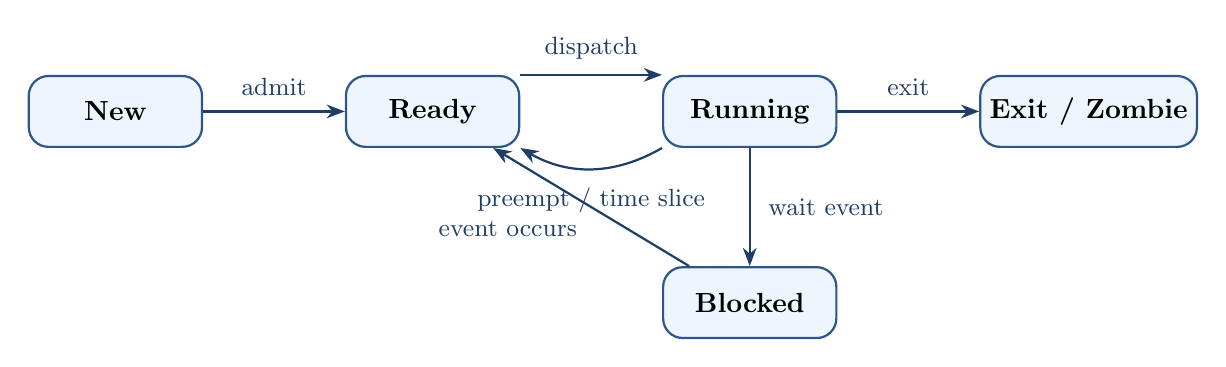
\begin{tikzpicture}[>=Stealth, node distance=1.4cm and 1.8cm]
\tikzset{
  state/.style={draw=mainblue, thick, fill=softblue, rounded corners=2.5mm, align=center, minimum width=2.2cm, minimum height=0.9cm, font=\bfseries}
}
\node[state] (new) {New};
\node[state, right=of new] (ready) {Ready};
\node[state, right=of ready] (run) {Running};
\node[state, below=1.5cm of run] (block) {Blocked};
\node[state, right=of run] (term) {Exit / Zombie};

\draw[->, thick, deepblue] (new) -- node[above=2pt, font=\small] {admit} (ready);
\draw[->, thick, deepblue] (ready.north east) -- node[above=2pt, font=\small] {dispatch} (run.north west);
\draw[->, thick, deepblue] (run.south west) to[out=210, in=330] node[below=3pt, font=\small] {preempt / time slice} (ready.south east);
\draw[->, thick, deepblue] (run) -- node[right=3pt, font=\small] {wait event} (block);
\draw[->, thick, deepblue] (block) -- node[below left=2pt, font=\small] {event occurs} (ready);
\draw[->, thick, deepblue] (run) -- node[above=2pt, font=\small] {exit} (term);
\end{tikzpicture}
\endgroup
\end{center}

\begin{corebox}[状态转换的第一原则]
\kw{每条状态箭头都必须有事件依据。} 如果说不出事件，就不应随意改变状态。
\end{corebox}

\subsection{阶段 A：创建——从父进程产生新执行环境}

Unix/POSIX 语义中，\code{fork()} 创建子进程。关键不是“复制所有物理内存”，而是创建一个新的进程语义实体，并让其初始状态看起来接近父进程。

现代实现常通过 COW 优化：
\[
\text{初始共享物理页}+\text{只读保护}\xrightarrow{\text{首次写}}\text{复制对应页}
\]

文件资源则有另一套语义：父子有各自 fd 表副本，但对应 fd 可以指向同一个 open file description。

\subsection{阶段 B：exec——不是新建进程，而是替换进程映像}

\code{exec()} 最应该记住一句：
\[
\boxed{\text{same process identity, new program image}}
\]
典型结果：
\begin{itemize}
\item 进程 PID 不因为 exec 本身变成另一个新 PID；
\item 原有代码、数据、栈等程序映像被新的可执行程序替换；
\item 未设置 close-on-exec 的打开文件描述符可以跨 exec 保留。
\end{itemize}

\subsection{阶段 C：Ready——只缺 CPU}

Ready 的精确定义不是“正在等待某事”，而是：
\[
\boxed{\text{运行所需条件已满足，只差 CPU 执行机会}}
\]
因此就绪队列中的实体如果此刻拿到 CPU，就能继续执行。

\subsection{阶段 D：Running——用户态和内核态都可能属于“这个进程正在运行”}

当进程执行系统调用进入内核时，常常仍然是\kw{当前进程上下文}。

因此：
\[
\text{Running}\not\equiv\text{User Mode}
\]

进程可以在内核中替自己执行系统调用处理，随后返回用户态；也可以在内核中发现条件不满足并进入阻塞。

\subsection{阶段 E：Blocked——即使给 CPU 也不能继续}

Blocked 与 Ready 的核心区别：

\begingroup
\small
\renewcommand{\arraystretch}{1.25}
\setlength{\tabcolsep}{6pt}
\begin{tabularx}{\linewidth}{>{\bfseries}p{0.26\linewidth} X X}
\toprule
对比维度 & 就绪态 (Ready) & 阻塞态 (Blocked)\\
\midrule
缺少的核心资源 & 只缺 CPU 时间片 & 缺少特定的外部事件或资源条件\\
给 CPU 能否继续运行 & 能立即投入 Running 运行 & 不能，即使分配 CPU 也无法向前推进\\
进入触发原因 & 被抢占、刚创建完成、从 Blocked 被唤醒 & 等待磁盘 I/O、信号量 P 操作、子进程退出等\\
离开触发原因 & 调度器选择 (Scheduler Pick) & 所等待的外部事件/资源就绪\\
\bottomrule
\end{tabularx}
\endgroup

\begin{warn}[“调用 read 就 Running→Blocked”也是过度简化]
\code{read()} 如果数据已经在缓存/缓冲中，可能直接完成并返回。只有在当前语义要求等待且数据尚未可用时，执行实体才可能睡眠/阻塞。类似地，用户态 mutex 的无竞争获取甚至可能不需要系统调用。
\end{warn}

\subsection{阶段 F：Wakeup——Blocked → Ready，不等于马上 Running}

设备完成、中断到来、条件被满足后，内核通常只是把等待实体变成 runnable/ready：
\[
\boxed{Blocked\rightarrow Ready}
\]
它仍然要等待 scheduler 选择：
\[
\boxed{Ready\rightarrow Running}
\]

这是 408 状态题最关键的两步分离。

\subsection{阶段 G：Exit / Zombie / Wait}

进程执行 \code{exit()} 后，绝大多数运行资源会释放，但 Unix 风格系统通常保留少量退出状态，供父进程通过 \code{wait()} 回收，因此出现 zombie 概念。

应理解为：
\[
\text{Process Execution Ends}\neq\text{All Kernel Metadata Immediately Vanishes}
\]

\section{调度：控制权已经回到内核，下一步给谁？}

\subsection{机制与策略必须拆开}

\begin{corebox}[机制 / 策略]
\textbf{机制（mechanism）}：OS 有没有能力停止当前执行流、保存状态、切换到另一个执行流？\\
\textbf{策略（policy）}：面对多个 runnable 实体，应该选择谁？
\end{corebox}

例如：
\[
\text{Timer Interrupt + Context Switch Machinery}=\text{Mechanism}
\]
而：
\[
\text{FCFS/SJF/RR/Priority/MLFQ}=\text{Policy}
\]

\subsection{调度评价指标是互相冲突的目标函数}

\begin{itemize}
\item CPU utilization：尽量别让 CPU 闲；
\item Throughput：单位时间完成更多工作；
\item Turnaround time：提交到完成；
\item Waiting time：在 ready queue 中等待的时间；
\item Response time：从请求到首次响应；
\item Fairness：避免长期得不到 CPU；
\item Predictability / deadline：实时系统特别关注。
\end{itemize}

不存在对所有工作负载同时最优的单一调度策略。

\subsection{经典算法应按“偏好谁”来记}

\begingroup
\small
\renewcommand{\arraystretch}{1.25}
\setlength{\tabcolsep}{5pt}
\begin{tabularx}{\linewidth}{>{\bfseries}p{0.14\linewidth} p{0.22\linewidth} X X}
\toprule
算法 & 核心偏好 & 主要优点 & 核心代价 / 潜在风险\\
\midrule
FCFS & 先到先服务 & 实现简单、低调度系统开销 & Convoy Effect（护航效应），短任务久等\\
SJF & 短 CPU Burst 优先 & 理论上可获得最小平均等待时间 & 难准确预测下一步 Burst，长任务易饥饿\\
SRTF & 剩余时间短者优先 & 抢占式偏向短任务，降低响应时间 & 频繁抢占与上下文切换开销大\\
Priority & 优先级高者优先 & 直观表达任务重要程度 & 低优先级任务长时期饥饿（需 Aging 机制）\\
RR & 人人轮流切时间片 & 响应极佳、保证公平性 & 时间片 $q$ 过小导致频繁切换；过大退化为 FCFS\\
MLFQ & 用历史行为推断类型 & 兼顾短交互任务与长计算任务 & 规则复杂，需要防范 Task Gaming 与饥饿\\
\bottomrule
\end{tabularx}
\endgroup

\begin{warn}[教材模型 vs 现代 Linux 调度算法]
MLFQ 是 408 考纲常考的经典教学策略；现代 Linux 普通任务调度长期采用 CFS 的“公平 CPU”模型，当前内核正在向 EEVDF 方向演进。备考时需以经典 MLFQ 规则为准，理解现代算法对公平性的优化。
\end{warn}

\subsection{时间片到底解决什么}

时间片不是越小越公平就越好：
\[
q\downarrow\Rightarrow Response\ may\ improve,
\quad ContextSwitchOverhead\uparrow
\]
\[
q\uparrow\Rightarrow Overhead\downarrow,
\quad RR\rightarrow FCFS
\]

因此调度本质上是：
\[
\boxed{\text{Latency}\leftrightarrow\text{Throughput}\leftrightarrow\text{Fairness}\leftrightarrow\text{Overhead}}
\]

\section{上下文切换：到底切了什么？}

\subsection{抽象定义}

上下文切换至少包括：
\begin{enumerate}
\item 保存旧执行实体下一次继续所需的 CPU 执行状态；
\item 更新其调度/运行状态；
\item 选择新执行实体；
\item 恢复新实体的 CPU 状态；
\item 必要时切换地址空间/内存上下文；
\item 从新实体的正确位置继续执行。
\end{enumerate}

\subsection{同进程线程切换与跨进程切换}

同进程线程共享地址空间，因此通常无需更换整个地址转换上下文；跨进程切换往往还需要切换地址空间相关状态。

\begin{warn}[考点辨析：上下文切换与 Cache/TLB 刷新]
408 经典模型常把地址空间切换视为 TLB 需要刷新或重新建立有效翻译；但在现代 CPU 工程实现中，可通过 ASID / PCID 标签保留部分 TLB 项，不必简单一刀切清空。
\end{warn}

\subsection{真正的动态轨迹：A 切到 B}

比“保存 PCB → 恢复 PCB”更好的理解是：
\[
A_{user}\rightarrow A_{kernel}\rightarrow Scheduler\rightarrow B_{kernel}\rightarrow B_{user}
\]
其中 scheduler 本身运行在内核控制路径中。

\section{系统调用、中断、异常：控制流为什么会改变}

\subsection{一次系统调用的五阶段模板}

\begin{enumerate}
\item 用户代码准备参数；
\item 执行体系结构规定的 trap/syscall 指令；
\item 硬件保存足够的返回状态并进入内核入口；
\item 内核验证参数、执行服务；
\item 若可立即完成则 return；若必须等待，则阻塞当前实体并调度其他实体。
\end{enumerate}

因此系统调用有两条最重要分支：
\[
\boxed{\text{Fast: syscall}\rightarrow\text{return same task}}
\]
\[
\boxed{\text{Slow: syscall}\rightarrow\text{block}\rightarrow\text{schedule someone else}}
\]

\subsection{时钟中断为什么是抢占式调度的基础}

若用户程序不主动进入内核，定时器仍能周期性打断 CPU：
\[
User\rightarrow TimerInterrupt\rightarrow Kernel
\]
这使 OS 有机会：
\begin{itemize}
\item 记账；
\item 更新运行时间；
\item 判断时间片/优先级；
\item 必要时触发抢占和重新调度。
\end{itemize}

\subsection{设备中断：唤醒并不等于直接交 CPU}

典型 I/O 完成：
\[
Device\rightarrow Interrupt\rightarrow KernelHandler\rightarrow Wakeup(Task)
\]
关键状态变化通常只是：
\[
Blocked\rightarrow Ready
\]
之后是否立即抢占当前任务，取决于调度策略和系统状态。

\section{超级母题一：一个进程从 fork 到 wait 的一生}

\begin{corebox}[推荐课堂主线]
不要先给学生五态图。先让学生跟踪一个真实进程：\code{shell fork → child exec → schedule → syscall → block → wakeup → exit → parent wait}。五态图应当从这个动态故事中“长出来”。
\end{corebox}

\subsection{完整轨迹}

\begin{enumerate}
\item Shell 正在 Running。
\item Shell 调用 \code{fork()} 进入内核。
\item 内核创建 child 的管理状态、地址空间语义（常用 COW）和继承资源引用。
\item child 进入 Ready；parent 也可能继续 Ready/Running，谁先运行不由 \code{fork()} 本身保证。
\item child 被调度后运行，调用 \code{exec()}。
\item \code{exec()} 替换 child 的程序映像，但保持该进程身份；未 close-on-exec 的 fd 可继续存在。
\item 新程序运行并发起一个系统调用。
\item 若系统调用可立即完成：kernel → user，仍是同一进程。
\item 若必须等待 I/O：Running → Blocked，进入等待队列，调度器选择另一个 Ready 实体。
\item 设备完成，中断进入内核；等待条件满足后 child：Blocked → Ready。
\item child 某次再次被调度：Ready → Running。
\item child 最终 \code{exit()}，释放大量运行资源，留下退出状态成为 zombie（Unix 语义）。
\item parent 的 \code{wait()} 获取退出信息并完成最终回收。
\end{enumerate}

\section{超级母题二：一次阻塞 read 的一生}

假设进程 A 调用：
\begin{verbatim}
read(fd, buf, 4096)
\end{verbatim}
且数据当前无法立即取得。

\begin{enumerate}
\item A 在用户态运行。
\item 系统调用使 CPU 进入 A 的内核上下文。
\item 内核根据 fd 查 A 的文件描述符表。
\item fd 指向 open file description / Linux \code{struct file}，取得 offset 与对象引用。
\item VFS/具体文件系统沿 dentry/inode、缓存和块映射路径处理请求。
\item 数据若已经在缓存：走 fast path，复制/返回，A 不必阻塞。
\item 本题设定 cache miss 且需要设备 I/O：内核提交 I/O。
\item A 当前无法继续：Running → Blocked。
\item scheduler 选择 B，发生 context switch。
\item 设备通过 DMA/控制器完成数据传输，随后产生中断。
\item 内核中断处理路径完成请求并 wake A：Blocked → Ready。
\item A 并未必立即运行；等待调度。
\item A 再次 Running 后从原系统调用睡眠点继续，完成 \code{read()}，最终返回用户态。
\end{enumerate}

\begin{exam}[一题串起的考点]
一次阻塞 \code{read()} 可以同时考：系统调用、用户/内核态、fd、进程资源、运行/阻塞/就绪状态、调度、上下文切换、设备中断、DMA、文件缓存与唤醒。它应成为本模块综合训练的第一母题。
\end{exam}

\section{线程实现模型：考试模型与现代实现边界}

\subsection{用户级线程与内核级线程真正区别：谁看得见、谁调度}

\begingroup
\small
\renewcommand{\arraystretch}{1.25}
\setlength{\tabcolsep}{6pt}
\begin{tabularx}{\linewidth}{>{\bfseries}p{0.26\linewidth} X X}
\toprule
对比维度 & 用户级线程 (ULT) & 内核级线程 (KLT)\\
\midrule
调度掌控者 & 用户态线程库 / 运行时 (Runtime) & OS 内核调度器\\
内核视角透明度 & 内核完全不可见（仅看到承载进程） & 内核直接感知并维护每条线程状态\\
切换是否进内核 & 无须内核参与，纯用户态上下文切换 & 必须经过中断/Trap 进入内核态完成切换\\
多核利用能力 & M:1 模型无法利用多核并行执行 & 可直接在多核 CPU 上同时调度并行执行\\
阻塞调用的影响 & 一个 ULT 发起阻塞系统调用拖垮整个进程 & 一个 KLT 阻塞不影响同进程其他 KLT 运行\\
\bottomrule
\end{tabularx}
\endgroup

\subsection{M:1、1:1、M:N 的本质}

它们讨论的是：
\[
\boxed{\text{User Execution Contexts}\rightarrow\text{Kernel Schedulable Contexts}}
\]
如何映射。

现代 Linux POSIX 线程通常采用 1:1 内核线程模型；Go goroutine、某些语言虚拟线程等则在语言运行时层面重新引入 M:N 式用户级调度思想。

\section{408 做题协议：从“概念题”升级为状态推演}

\subsection{进程状态题六问}
\begin{enumerate}
\item 当前实体是 Ready、Running 还是 Blocked？
\item 它缺的是 CPU 还是外部事件？
\item 发生了什么事件？
\item 事件只改变状态，还是还会触发调度？
\item 唤醒后是否只是进入 Ready？
\item 是否混淆“进程在内核态执行”和“换成另一个进程”？
\end{enumerate}

\subsection{调度计算题六步}
\begin{enumerate}
\item 写出 arrival time、burst time、priority、quantum 等输入；
\item 确定抢占/非抢占；
\item 每个关键事件点重新确定 ready set；
\item 按策略选择；
\item 画 Gantt 图；
\item 从完成时刻反推 turnaround / waiting / response，最后检查单位与定义。
\end{enumerate}

\subsection{系统调用/中断题七问}
\begin{enumerate}
\item 入口是 syscall、exception 还是 interrupt？
\item 是同步还是异步？
\item CPU 是否进入内核态？
\item 当前还是原进程上下文吗？
\item 当前任务能否继续？
\item 若不能，进入哪个等待队列/状态？
\item 最终是 return same task，还是 schedule another task？
\end{enumerate}

\subsection{文件描述符/fork 题五问}
\begin{enumerate}
\item fd 表是各自复制还是同一张？
\item 两个 fd 是否指向同一个 open file description？
\item 文件 offset 是共享还是独立？
\item 最终是否指向同一个 inode/filesystem object？
\item 操作是 \code{open}、\code{dup}、\code{fork} 还是 \code{exec}？四者的共享语义不同。
\end{enumerate}

\section{本模块的知识树与后续接口}

\begin{center}
\begin{tikzpicture}[>=Stealth,node distance=7mm and 9mm,scale=.93,transform shape]
\tikzstyle{n}=[draw,rounded corners,align=center,minimum width=28mm,minimum height=8mm]
\node[n,fill=softblue] (ctrl) {控制权\\user/kernel, trap};
\node[n,below left=of ctrl,fill=softgreen] (proc) {执行抽象\\process/thread};
\node[n,below right=of ctrl,fill=softgreen] (event) {事件入口\\syscall/exception/IRQ};
\node[n,below=14mm of ctrl,fill=softorange] (life) {生命周期\\ready/run/block/exit};
\node[n,below left=of life] (sched) {调度\\policy + context switch};
\node[n,below right=of life] (res) {资源引用\\address space + fd};
\node[n,below=of life,fill=softred] (next) {后续模块\\并发 / 虚存 / I/O / 文件系统};
\draw[->] (ctrl)--(proc);\draw[->](ctrl)--(event);
\draw[->](proc)--(life);\draw[->](event)--(life);
\draw[->](life)--(sched);\draw[->](life)--(res);
\draw[->](sched)--(next);\draw[->](res)--(next);
\end{tikzpicture}
\end{center}

\begin{corebox}[最终应形成的心智模型]
这一模块学完，学生看到“进程”时不应只想到 PCB；而应自动看到：
\[
\boxed{
\text{Resource Context}
+
\text{Execution Context}
+
\text{Kernel State}
}
\]
看到“状态变化”时应自动问：
\[
\boxed{\text{什么事件？谁获得控制？当前还能继续吗？}}
\]
看到“调度”时应自动区分：
\[
\boxed{\text{Mechanism}\neq\text{Policy}}
\]
看到 \code{read/fork/exec} 时则应能沿着进程生命周期和资源引用图完整推演。
\end{corebox}

\section*{参考与工程校准来源}
\addcontentsline{toc}{section}{参考与工程校准来源}
\begin{itemize}
\item Remzi H. Arpaci-Dusseau, Andrea C. Arpaci-Dusseau, \emph{Operating Systems: Three Easy Pieces}：进程、受限直接执行、调度与并发的教学框架。
\item MIT PDOS, \emph{xv6: a simple, Unix-like teaching operating system}：trap、scheduler、sleep/wakeup、process lifecycle 的实现级案例。
\item POSIX / The Open Group：\code{fork()}、\code{open()}、\code{dup()}、\code{exec()} 对文件描述符/open file description 的规范语义。
\item Linux Kernel Documentation：VFS 的 dentry/inode/file object 模型，以及 CFS/EEVDF 调度器的工程实现边界。
\end{itemize}

\end{document}
